%Empieza configuracion de capitulo

\setstretch{1.0}
\titleformat{\chapter}[block]{\Large\bfseries}{CHAPTER 
\Huge\thechapter\vspace{25 pt}}{0 pt}{\\\fontsize{26}{36}\selectfont}
\titlespacing{\chapter}{0 pt}{30 pt}{50 pt}[0 pt]
\titleformat{\section}{\Large\bfseries}{\thesection}{0 pt}{\hspace{30 pt}}
\titleformat{\subsection}{\large\bfseries}{\thesubsection}{0 pt}{\hspace{30 pt}}
\pagestyle{fancy}
\fancyhead[LO,LE]{\footnotesize\textit{\leftmark}}
\fancyhead[RO,RE]{\thepage}
\fancyfoot[CO,CE]{}
%Termina configuracion de capitulo

\chapter{Introduction} %Cambia Introducci'on al nombre de tu capitulo
\setstretch{1.5} %Regresa el interlineado a 1.5

\normalsize

This work Will present a detailed study of how could a network of embedded
systems collaborate among each others to solve parallel problems. After reading
this project you will understand how this can be done , what are their
limitations and recommendations if you would like to implement this as part of 
your current projects. 

\section{Background}
\vspace{30 pt}
\noindent

Our story begins decades ago, the computers were finally at homes and many
people wonder what was going to be next revolution. There was expectations that
in close future the Computers were going to be everywhere: in our houses , in
our cars, teaching to the children and controlling the traffic. Well that was
the dream that seems more like a science fiction story, but as we know that
dream has came true in many ways.

All this has been possible due to the evolution of computing technology over
these years. Computer technology has made incredible progress in the roughly 60
years since the first general-purpose electronic computer was created. Today,
less than 500 dollars  will purchase a personal computer that has more
performance, more main memory, and more disk storage than a computer bought in
1985 for 1 million dollars.\cite{Hennessy} This rapid improvement has come both
from advances in the technology used to build computers and from innovation in
computer design.

The 1980s saw the rise of the desktop computer based on microprocessors, in the
form of both personal computers and workstations. The 1990s saw the emergence
of the Internet and the World Wide Web, the first successful hand-held computing
devices, and the emergence of high-performance digital consumer electronics.
The extraordinary popularity of cell phones has been obvious since 2000, with
rapid improvements in functions and sales that far exceed those of the PC.
These more recent applications use embedded computers.

But let's stop a bit here. A new world came to our vocabulary at those days:
embedded. What is an embedded system? An embedded system is a special-purpose
system in which the computer is completely encapsulated by the device it
controls.\cite{Hallinan} Unlike a general-purpose computer, such as a personal
computer, an embedded system performs pre-defined tasks, usually with very
specific requirements. Examples of these was the first microwaves, the first
cellphones and GPS systems. All those electronic gadgets that started to emerge
10 years ago.

As we know society loved these new devices and asked for more. Less cost,
smaller devices, better power consumption and the capability to make much more
complex tasks. This was a clear path to follow until a new requirement came up:
Connectivity. The market started to ask for embedded systems with the
capability,not only to measure, but also with the capability to be fully
connected to the internet all the time. One could start to ask why. Why would I
want to have an embedded system connected to the internet all the time?. Can
you imagine now your TV, smart phone or tablet not connected to the Internet?
This is the technology that old science fiction novels imagined years ago, the
internet of things.

Internet of Things (IoT) refers to physical and virtual objects that have
unique identities and are connected to the internet to facilitate intelligent
applications that make energy, logistics, industrial control, retail,
agriculture and many other domains "smarter".\cite{Bahga} The IoT enables the
interconnection via the Internet of computing devices embedded in everyday
objects, enabling them to send and receive data. So what is the diference
betwen the embddded systems and the IoT systems? As you can see the differences
with traditional embedded systems are the internet connectivity and less power
consumption. IoT systems must always be connected to the internet and require a
lower power consumption.

But the entire picture of an IoT solution is quite bigger. A full solution has 
the following parts (figure~\ref{fig:1.1}).

\begin{itemize} 

\item The Thing (computing devices):  in the Internet of
Things, can be a person with a heart monitor implant, a farm animal with a bio
chip transponder, an automobile that has built-in sensors to alert the driver
when tire pressure is low or any other natural or man-made object that can be
assigned an IPA address and provided with the ability to transfer data over a
network 

\item Network Connection: Network Connections provides connectivity
between your computing devices  and the Internet, a network, or another compute
device 

\item Cloud computing Data centers for storage and Big Data analysis: The data
by itself is not useful to the end user. An alarm or recommendation is all that
the end user will matter. After the data is sent and stored into the Cloud
Computing Data Centers is necessary to run Big Data solutions that present
meaning full information to the users.  

\item Presentation Devices: At the end of the day, what do we do with all that
information we have collected?; one obvious thing is to display the information
via a dashboard. Dashboards have to be hosted on some kind of display, we call
that the Presentation Device.  It could be a desktop computer running an 
application, a tablet or a smart phone accessing to a web page. It could
even be a purpose-built device like a retail kiosk, intelligent vending machine
or a control panel. The goal is to present the information coming from the big
data analysis.

\end{itemize}

\begin{figure}[H]
\centering
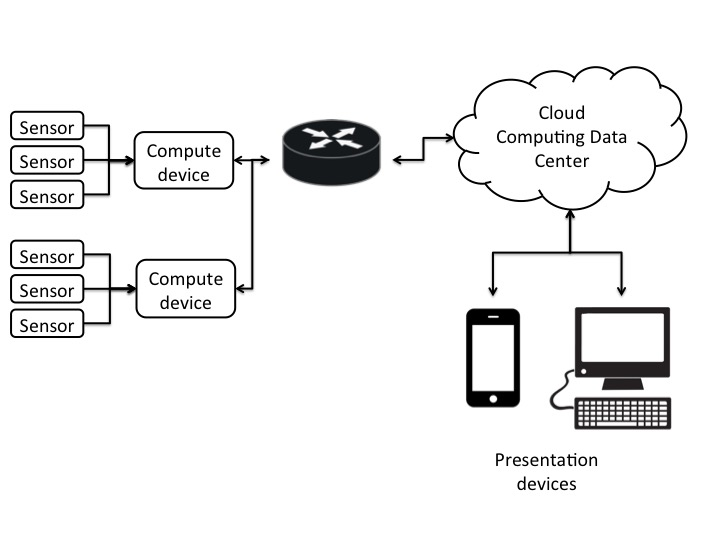
\includegraphics[width=0.75\textwidth]{images/IoT_diagram.jpg}
\caption{IoT full diagram }
\label{fig:1.1}
\end{figure}

Like many booming areas of technology, the internet of things revolution is
plagued by a lack of industry standards. As you can imagine there are thousands
of computing devices and sensors from different vendors that appear on the
market  every day , each one with his unique way to send  or store their data
in their centralized cloud computing centers.

Right now exist two main projects that are compiling to establish standards for
the IoT communications: 

\begin{itemize}
\item Open Interconnect Consortium (OIC): OIC is an industry group whose stated 
mission is to develop standards and certification for devices involved in the 
Internet of Things based around CoAP. OIC was created in July 2014 by Intel, 
Broadcom, and Samsung Electronics.\cite{OIC}

\item AllJoyn : AllJoyn is an open, universal, secure and programmable software 
connectivity and services framework that enables companies and enterprises to 
create inter-operable products that can discover, connect and interact directly 
with other AllJoyn-enabled products. \cite{AllJoyn}
\end{itemize}


Both standards try to solve a simple problem. Imagine you have smart light bulbs
in your house, all of them a device of your IoT network at home. What happened
if one of them burns? You go and buy one but then you remember that all your
light bulbs at home are brand A and at the store there are only brand B
light bulbs. It should be possible to bring any brand of light bulbs and
still work with the rest of the devices of your network. This will be possible
with communications standards among the industry.These two efforts are fighting
each other to generate these kind of standards in IoT communications. Which one
is the best ? maybe is too soon to have a winner, but in less than a decade
this question might be answered. 

In the meantime the Internet of Things revolution is here whether we like it or
not. We live in houses with computers inside our air conditions, televisions
and cars; many of them connected to the internet, but as we have seen there are
parts that are being missing. Despite the efforts to develop standard network
protocols for IoT systems there is no effort to make the IoT systems analyze
their data among each others instead of send  all the data to Cloud Data
centers to be analyzed. This could be a problem in a short future because as we
have we will the solution is not to add another server (specially when you have
space and economic constrains)


\section{Problem Definition}
\noindent

In order to understand the severity of the problem we have to understand the
magnitude of it, we have to understand that the rise of the internet of things
is real.  According to a study by the International Data Corporation (IDC)
\cite{IDC}, a market research analysis and advisory firm specialized in
information technology estimate the number of IoT devices is approaching  200
billion. And the number of sensors that track, monitor, or feed data to those
things is already more than 50 billion, with scientists talking about
trillion-sensor networks within 10 years. Of course, not all of those 200
billion things are actually wired and communicating on the Internet, but some
20 billion are. And, by 2020, this number will grow by 50\% to 30 billion
connected devices.\cite{EMC1}

But the rise of the internet of things means the rise of data. Imagine for a
moment that the 20 billion of devices try to send 1 kilobyte of data to the
centralized servers, this will create so much traffic that might be similar to
a security attack, collapsing the centralized data centers. One could imagine
that this is not a problem, that we might be exaggerating; but as we saw there
are actual problems like the one Virgin Atlantic airline has.

In 2014 the Boeing 787 aircraft ordered by Virgin Atlantic for delivery
dramatically increases the volume of data the airline will need to deal with
(half terabyte in a transatlantic flight). \cite{Finnegan} Because they can't
handle that much terabytes of data everyday coming from various airplanes they
are looking for cloud base solutions inside the airplanes. Now consider that
the space in an airplane is limited and expensive, moreover the electric
energy. A cloud base solution (adding servers inside the airplane) will require
both space and electric energy.

Besides that, the power consumption of these  IoT's Cloud Data Centers is a key
part to considerate. If current trends continue, a petaflop system will require 
100 megawatts to manage the IoT data \cite {Xizhou} (imagine that power
consumption in an airplane)

The rise of IoT will lead to an explosion in the volume of data collected,
transmitted and processed.This will require novel and optimized solutions.  How
can we make the IoT networks self sustainable? Make them solve their own
compute problems without the need to send millions of data to the cloud data
centers?. How can we know when is really necessary to send the data to the cloud
data centers because the number of IoT systems is not efficient ( in terms of
energy and performance)? What kind of applications are good candidates for
these kind of solution? All these questions will be addressed in this work. 

\section{General Objective}
\noindent

The main objective is to find the maximum number of low ultra-low-voltage
microprocessors platforms that provides the maximum level of energy efficiency.

After finding this information for commons benchmarks it will be easy for the
industry of IoT systems to determine if their applications can take advantage
of communicate their IoT devices to process their own data instead of sending
the information to data centers.

\section{Hypothesis}
\noindent

We are confident that with the current technology is possible to generate a
distributed system of ultra-low-voltage microprocessors platforms (core
systems of the IoT devices). The part that we are concern is determine the
breaking point where is better to send the data to the cloud data centers. How
many systems is the maximum that these kind of network could support and still
being a good option in terms of energy efficiency?

In computing, performance per watt is a measure of the energy efficiency of a
particular computer architecture or computer hardware. Literally, it measures
the rate of computation that can be delivered by a computer for every watt of
power consumed.\cite{Burd} 


\begin{equation}
    Energy Efficiency = \dfrac {Performance}{Watts}
\end{equation}

We believe that the energy efficiency in an embedded cluster will have the
behavior of the  figure~\ref{fig:1.2}. in the beginning the increment of the
number of nodes in our network will increment the performance (the top part of
the equation), but at the same time the amount of watts will
increase making the energy efficiency flat at some point (if the lower part of
the equation increases the equation tends to decrease)


\begin{figure}[H]
\centering
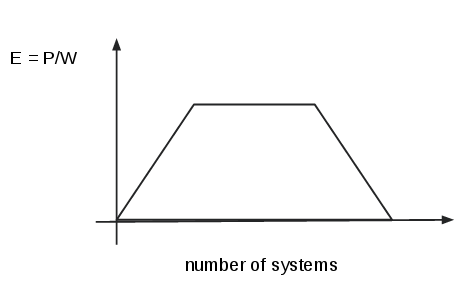
\includegraphics[width=0.75\textwidth]{images/graph_1.png}
\caption{Hypothesis of energy efficiency behavior in embedded cluster}
\label{fig:1.2}
\end{figure}

After finding these curves for command benchmarks it will be easy for the
industry of IoT systems to determine if their applications can take advantage
of communicate their IoT devices among each others instead of sending the
information to their data centers.


\section{Methodology}
\noindent

Recent researches \cite{Saldana} \cite{Gallego} \cite{McMahon} \cite{Liu} are 
showing an increasing interest in the topic.  All these research always talk
about the lack of three parts: 

\begin{itemize}
\item A low-voltage microprocessors platform with enough compute power
\item An operating system for Distributed Systems
\item A light communication protocol to distribute the workload among the
embedded platforms
\end{itemize}

The way we are going to address this will be:


\begin{itemize}

\item Chose the right embedded platform: There are dozens of embedded and IoT
platforms, this is why is necessary to make a deep analysis and choose the best
platform that feed our needs. (taking into consideration that sometimes the
systems might have heterogeneous platforms)

\item Chose the right communication and compute protocol: There are different
kinds of distributed compute protocols. Part of this investigation is to detect
the most reliable and suitable for our needs.

\item Chose the right Operating System for the system. Once we have selected
the appropriate embedded platforms, another variable in this investigation is
the number of Operating Systems. Either if it is a micro kernel or a monolithic
kernel architecture there are more than a dozen of solutions to use.

\item Create embedded clusters to measure energy efficiency. Once we have found
the best configuration (Hardware + Operating System + Communication Protocol )
in terms of energy efficiency , we can start to create a cluster of embedded
systems.

\item Release all the improvements and disagreements found Open Source and
public. All the improvements made into any technology (operating systems or
communication protocols) will be published with an open source license.

\item Implement solution on real application ( greenhouse ). In order to test
or hypothesis in a real application we will implement it on a real greenhouse.
Proving that the solution give an embedded system the power of reliability and
availability without the need of external and expensive servers 
\end{itemize}


\clearpage
